
There has yet to be a true definition of what an agent is. A lot of different literatures define an agent in their own way.
All these definitions are strongly based on the background of the research they are conducting. By \citet{AI:agent}, an agent is defined as :

\begin{center}
    \textit{\textbf{"An agent is anything that can be viewed as perceiving its environment through sensors and acting upon that environment through effectors."}}
\end{center}


\begin{figure}[ht]
   \centering
   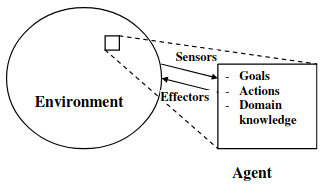
\includegraphics[scale=0.8]{env-agent.png}
   \caption[Agent]{How the environment can be perceived by an agent}
\end{figure}

This means that an agent is an entity that can perceive its environment through sensors and 
perform tasks using data received from these sensors. 

An agent has two basic properties, being autonomous and being situated in an environment \cite{AI:guide}. 
To achieve autonomy the entity must have a goal. An autonomous agent will try and achieve this goal using a set of actions. 
The agent will decide independently what the best set of actions is. During this process there will be no direct intervention from other entities.

To enable an agent to be situated it must have the ability to adapt to dynamic (changing rapidly, unpredictable (not static) 
and unreliable environments (it is not able to predict future states of the environment).

An intelligent agent has additional properties :

\begin{itemize}
   \item Reactive
   \item Proactive
   \item Flexible
   \item Robust
   \item Social
\end{itemize}

A dynamic environment is a repidly changing environment. An agent is often situated in a dynamic environment.
Because of this it will need to adapt to each change to keep pursuing the goal, the agent is reactive. 

The second additional property, proactive, is that the agent will keep pursuing the goal over time. 
If an attempt fails, the agent will need to recover and be robust. 
To achieve robustness the agent will need a range of actions to achieve 
the goal, so it can be flexible in case some actions are not available, have failed before. 

Lastly, an intelligent agent is able to interact with other agents and share its knowledge, the agent is social.